\documentclass[11pt,a4paper,oneside]{scrartcl}
\usepackage{requiredPackages}
\usepackage{subfig}
\usepackage{cancel}
\usepackage[labelfont=bf]{caption}
\usepackage{booktabs}
\interfootnotelinepenalty=10000

\def\UrlBreaks{\do/\do-\do_}
\begin{document}
\begin{titlepage}
	\centering
	{\scshape\LARGE Ludwig-Maximilians-Universität \linebreak München \par}
	\vspace{1cm}
	{\scshape\Large Fortgeschrittenenpraktikum II \par Wintersemester 22/23 \par}
	\vspace{1.5cm}
	{\huge\bfseries \par  Gaußsche Strahlenoptik\par}
	\vspace{2cm}
	{\Large\itshape Guido Osterwinter und Jan-Philipp Christ \par}
	\vfill
	{\large München, den \today\par}
\end{titlepage}

\tableofcontents
\newpage
\section{Zielsetzung}
Die geometrische Optik liefert nur eine unzureichende Beschreibung von Laserstrahlen, da im Rahmen dieser der Wellencharakter des Lichtes gänzlich vernachlässigt wird. Deutlich wird dies insbesondere bei konvergenten Strahlen, die nach der geometrischen Optik in einen einzelnen Punkt zusammenlaufen würden, obwohl dies durch Beugungseffekte nicht zulässig ist. \\
Berücksichtigt man nun den Wellencharakter des Lichtes und das typischerweise gauß-förmige Intensitätsprofil eines Laserstrahls, führt dies zur Gaußschen Strahlenoptik. \\
Im ersten Teil des hier vorgestellten Versuchs soll es um das experimentelle Untersuchen charakteristischer Größen eines solchen Laserstrahls gehen. So wird die Strahltaille (Waist) senkrecht zur Ausbreitungsrichtung sowie der Strahlradius als Funktion der zur Ausbreitungsrichtung parallelen Koordinate untersucht.\\
Im zweiten Versuchsteil wird das Verhalten Gaußscher Strahlen in einem aus zwei gekrümmten halbdurchlässigen Spiegel bestehenden Resonator untersucht. Insbesondere wird auf die Transmissionsfunktion als Funktion des Spiegelabstandes eingegangen und beispielhaft die Finesse eines konfokalen Resonators bestimmt. 
\section{Theoretischer Hintergrund}
\subsection{Gaußstrahlen}
\subsubsection{Ideale Gaußstrahlen}
Die Darstellung in diesem Abschnitt stützt sich, sofern nicht anders angegeben, auf Abschnitt 1 aus \cite{versuchsanleitung}. \\
Für monochromatische Lichtfelder linearer Polarisation der Form 
\begin{equation}\label{E_vec}
\vec E(\vec x,t)=\vec e\cdot E(x,y,z)\cdot e^{i\omega t}
\end{equation}
wird die elektromagnetische Wellengleichung in homogenen Medien zu
\begin{equation}\label{wave_eq}
\left(\frac{\partial^2}{\partial x^2}+\frac{\partial^2}{\partial y^2}+\frac{\partial^2}{\partial z^2}+k^2\right)E(x,y,z)=0
\end{equation}
Breitet sich ein Lichtfeld entlang der z-Richtung aus, so vereinfacht sich die Ortsabhängigkeit der Amplitude in \ref{E_vec} zu 
\begin{equation}\label{E_ansatz}
E(x,y,z)=E_0X(x,z)Y(y,z)e^{-ikz}.
\end{equation}
Nun sind häufig nur Strahlen von Interesse, die der schon aus der geometrischen Optik bekannten paraxialen Näherung genügen. Dies umfasst Strahlen, die sich nah an der optischen Achse bewegen und mit dieser nur kleine Winkel einschließen. Somit verschwinden für solche Strahlen in guter Näherung die zweiten partiellen Ableitungen nach $z$, da diese, wenn sie nicht $0$ wären, ein \glqq Wegkrümmen\grqq\ des Strahls von der optischen Achse beschreiben würden.\\
Einsetzen von \ref{E_ansatz} in \ref{wave_eq} liefert mit $X\equiv X(x,z), Y\equiv Y(y,z)$:
\begin{align}
0&=\left(\frac{\partial^2}{\partial x^2}+\frac{\partial^2}{\partial y^2}+\frac{\partial^2}{\partial z^2}+k^2\right)E(x,y,z) \\ \quad&
=\left(\frac{\partial^2}{\partial x^2}+\frac{\partial^2}{\partial y^2}+k^2\right)E(x,y,z)+\partial_z\left(-ikE_0XYe^{-ikz}+E_0e^{-ikz}\partial_z(XY)\right) \\ \quad&
=\left(\frac{\partial^2}{\partial x^2}+\frac{\partial^2}{\partial y^2}+\cancel{k^2}\right)E(x,y,z)-\cancel{k^2E_0XYe^{-ikz}}-2ikE_0\partial_z(XY)e^{-ikz}\\ \quad& -ikE_0e^{-ikz}XY+E_0e^{-ikz}\underbrace{\partial_z^2(XY)}_{\approx 0}
\end{align}
Man überzeugt sich nun nach einmaligem Anwenden der Produktregel auf den Term mit $\partial_z$ schnell davon, dass für nicht-triviale $X,Y$ gelten muss:
\begin{equation}
\left(\frac{\partial^2}{\partial x^2}-2ik\frac{\partial}{\partial z}\right)X(x,z)=\left(\frac{\partial^2}{\partial y^2}-2ik\frac{\partial}{\partial z}\right)y(y,z)=0
\end{equation}
Lösungen hiervon sind die Hermite-Gaußschen $\mathrm{TEM}_{m,n}$ Moden. Dabei beschreiben $n,m\in\N$ die Anzahl von Knoten im axialen Intensitätsprofil in $x-$ respektive $y-$Richtung.\\
Die Stärke der Divergenz dieser Moden wird bestimmt durch den Waist $w_0$, der auch die sogenannte Rayleigh-Länge \begin{equation}\label{rayleigh} z_R\equiv \frac{\pi w_0^2n}{\lambda}\end{equation}festlegt. Der Strahlradius nimmt entlang der Ausbreitungsrichtung die folgende Form an ($z_0$ ist der Ort, an dem die Waist angenommen wird):
\begin{equation}
\label{transv_profil}
w(z)=w_0\sqrt{1+\frac{(z-z_0)^2}{z_R^2}}
\end{equation}
Wie sich herausstellt, beschreibt das Wertepaar $(w_0,z_R)$ und damit auch die Größe $q\equiv w_0+iz_R$ einen Gaußstrahl vollständig.\\
Wird nun ein optisches System durch eine Transfermatrix \begin{equation}
T\equiv\begin{bmatrix}
A& B\\
C & D
\end{bmatrix}
\end{equation}
beschrieben- zur Berechnung von Transfermatrizen für einige konkrete Systeme vergleiche beispielsweise \cite{demtröder_2}- so werden $w_0$ und $z_R$ gemäß dem sogenannten 'ABCD'-Gesetz für Gaußstrahlen transformiert:
\begin{equation}\label{ABCD-Gesetz}
q^\prime = \frac{Aq+B}{Cq+D}
\end{equation}
\subsubsection{Reale Gaußstrahlen}
Reale (Laser-)Strahlen lassen sich natürlich nur in einem gewissen Maße als ideale Gaußstrahlen beschreiben. Um dem Verhalten realer Gaußstrahlen Rechnung zu tragen, führt man die dimensionslose Beugungsmaßzahl $M^2$ ein (vgl. \cite{paschotta2016m2}). Es ist für Gaußstrahlen $M^2=1$ und allgemein $M^2\geq 1$. Ein realer Strahl weitet sich gemäß dem Zusammenhang
\begin{equation}\label{rayleigh_m2}
z_R=\frac{w_0^2\pi n}{\lambda}\cdot \frac1{M^2}
\end{equation}
schneller auf als ein idealer Gaußstrahl. Da nach Gleichung \ref{ABCD-Gesetz} $z_R$ nicht durch ideale optische Elemente wie Linsen verändert wird, ist auch $M$ invariant unter idealen optischen Elementen. Dieser Umstand wird später noch aufgegriffen.
\subsubsection{Beispiel für Anwendung des 'ABCD'-Gesetzes}
\image{Skizze_A1}{Fokussierung eines Gaußstrahls auf bestimmten Waist $w^\prime_0$}{1}{Skizze_Aufgabe_S7.png}
Gegeben zwei Konvexlinsen mit Brennweiten $f_1,f_2$ soll ein Laserstrahl, dessen Waist $w_0$ anfangs in der ersten Linse sei, auf den Waist $w_0^\prime$ präpariert werden. Hierfür soll der Abstand $d$ zwischen den beiden Linsen bestimmt werden.\\
Gegeben sind die Werte $w_0 = 1\ \mathrm{mm}$, $\lambda = 632.8\ \mathrm{nm}$, ${w'}_0 = 5 \mu \mathrm m$, $f_1 = 50\mathrm{mm}$, $f_2 = 100\ \mathrm{mm}$. Um hieraus $d$ zu bestimmen, betrachte man die Transfermatrix
\begin{equation}
\begin{bmatrix}
    1 & 0 \\
    -\frac{1}{f_2} & 1 
\end{bmatrix}
\cdot
 \begin{bmatrix}
    1 & d \\
    0 & 1 
\end{bmatrix}
\cdot
 \begin{bmatrix}
    1 & 0 \\
    -\frac{1}{f_1} & 1 
\end{bmatrix}
\,\,=\,\,
 \begin{bmatrix}
   1-\frac{d}{f_1} & d \\
    \frac{d-f_1-f_2}{f_1 f_2} & 1-\frac{d}{f_2} 
\end{bmatrix}
\equiv
 \begin{bmatrix}
   A & B \\
    C & D 
\end{bmatrix}
\end{equation}
Für die Umgebung, in der sich die Gaußstrahlen ausbreiten, sei in guter Näherung ein Brechungsindex von $n=1$ angenommen. Der Wert von $q$ in Abbildung \ref{Skizze_A1} ist dann
\begin{equation}
q \,\,=\,\, 0 + i \frac{\pi}{\lambda} w_{0}^2
\end{equation}
Gemäß dem 'ABCD'-Gesetz für Gaußstrahlen gilt damit für $q'$ in Abbildung \ref{Skizze_A1} Gleichung \ref{ABCD-Gesetz}.\\
Für $q'$ soll aber auch
\begin{equation}\label{Gl2}
q' \,\,=\,\, -f_2 + i \frac{\pi}{\lambda} {w'}_{0}^{2}
\end{equation}
gelten. Aus den Gleichungen \ref{ABCD-Gesetz} und \ref{Gl2} nach $d$ auf, erhält man für $d$ die definierende Gleichung
\begin{align}
\left( f_1 f_2 \frac{w_0}{{w'}_{0}} \right)^2 \,\,&=\,\, \left( f_1 f_2 - d f_1 \right)^2 + \left( d - f_1 - f_2 \right)^2 \cdot \left(\frac{\pi w_{0}^{2}}{\lambda} \right)^2\\ \quad&
\Rightarrow \,\,\,\, d \,\,=\,\, 35.14\ \mathrm{cm}
\end{align}
Eine analoge Rechnung bei $f_2\leftrightarrow f_1$ liefert mit $d=35.13\ \mathrm{cm}$ nahezu den identischen Wert.
\subsection{Optische Resonatoren}
Auch die Darstellung in diesem Abschnitt stützt sich, sofern nicht anders angegeben, auf Abschnitt 1 aus \cite{versuchsanleitung}. \\
Ein optischer Resonator ist ein Paar aus halbdurchlässigen Spiegeln, in Abhängigkeit von deren Krümmungsradien $R$ und Abstand $L$ zueinander Randbedingungen für die transmittierten Moden festgelegt werden. Es gilt für die Strahltaille:
\begin{equation}
w_0^2=\frac{\lambda}{\pi}\sqrt{\frac{L}{2}\left(R-\frac{L}{2}\right)}
\end{equation}
Im Versuch wird ein symmetrischer Resonator verwendet, bei dem die Waist in der Mitte der Spigel liegt und die beiden Spiegel dieselben Krümmungsradien haben. Da zudem $L\approx R$ sein soll, spricht man von einer konfokalen oder zumindest nah-konfokalen Anordnung.\\
Im Wesentlichen ist auch von einem Resonator mit gekrümmten Spiegeln eine derjenigen eines planaren Fabry-Perot-Resonators ähnliche Transmissionsfunktion zu erwarten mit dem Unterschied, dass die Phasendifferenz nach einem Durchlauf i.A. nicht mehr nur von der Geometrie des Resonators, sondern beispielsweise auch von der eingekoppelten Mode abhängt. \\
Eine charakteristische Größe eines Fabry-Perot-Resonators ist die Finesse $F$ die das Verhältnis aus dem freien Frequenzbereich (Abstand zwischen zwei Resonanzpeaks) und der FWHM-Breite eines Resonanzpeaks beschreibt:
\begin{equation}
F\equiv \frac{\Delta \omega_{\mathrm{FSR}}}{\Delta \omega_{\mathrm{FWHM}}}
\end{equation}
Andererseits kann man zeigen, dass, wenn die beiden Spiegel die Reflektivitäten $R_1$ und $R_2$ haben, die folgende Beziehung zwischen der Gesamtreflektivität $R\equiv \sqrt{R_1R_2}<1$ und $F$ gilt:
\begin{equation}\label{finesse_theor}
F= \frac{\pi\sqrt{R}}{1-R}
\end{equation}
\subsubsection{Aufbau des verwendeten Resonators}
\image{Skizze_A2}{Aufbau zum optischen Resonator (aus \cite{versuchsanleitung}, bearbeitet)}{1}{Skizze_Aufgabe_S16.png}
\setcounter{figure}{3}
Damit sich im symmetrischen nah-konfokalen Resonator aus sphärischen Spiegeln eine stehende Welle bilden kann, soll die Waist des Gauß-Strahls mittig zwischen den beiden Spiegeln liegen. Betrachtet man den halbdurchlässigen Spiegel $\mathfrak{S}$, durch den der Gaußstrahl in den Resonator einfällt, als Linse der Dicke $b=6.35\ \mathrm{mm}$ und mit Krümmungsradien $R_1=\infty,R_2\equiv R=50\ \mathrm{mm}$, so kann unter Zuhilfenahme der Brechungsmatrix 
\begin{align}
B_R\equiv \begin{bmatrix}
1 & 0\\
\frac{n_1-n_2}{n_2\cdot R} & \frac{n_1}{n_2}
\end{bmatrix} 
\end{align}
an einer gekrümmten Ebene zwischen zwei Medien mit Brechungsindizes $n_1$ und $n_2$
nach \cite{dewiki:225621757} die Transfermatrix von $\mathfrak{S}$ bestimmt werden:
\begin{align}
T & \equiv
\begin{bmatrix}
A & B\\
C & D 
\end{bmatrix} 
\equiv
\begin{bmatrix}
1 & 0\\
\frac{n-1}{|R|} & \frac{n}{1}
\end{bmatrix} 
\cdot
\begin{bmatrix}
1 & b\\
0 & 1
\end{bmatrix} 
\cdot
\begin{bmatrix}
1 & 0\\
\frac{1-n}{n\cdot \infty} & \frac{1}{n}
\end{bmatrix} 
\\ \quad& = \begin{bmatrix}
1 & \frac{b}{n}\\
\frac{n-1}{R} & 1+\frac{b(n-1)}{nR}
\end{bmatrix}
\end{align}
Im Resonator geben die Randbedingungen vor, dass $w_0^\prime=\sqrt{\frac{\lambda}{\pi}\sqrt{\frac{d}{2}\left(R-\frac{d}{2}\right)}}$ gilt, wodurch insbesondere $q^\prime\equiv z^\prime+iz_R^\prime$ festgelegt wird. Damit lässt sich auf $q=z+iz_R$ außerhalb des Resonators, also vor dem Einkoppeln des Strahls in den Resonator, schließen:
\begin{align}
\ref{ABCD-Gesetz}& \iff q = \frac{Dq^\prime-B}{A-Cq^\prime}\\ & \Rightarrow z_R=\Im{q}=\Im{\frac{D\cdot (z^\prime+iz_R^\prime)-B}{A-C\cdot(z^\prime+iz_R^\prime)}}\\ \quad&=\Im{\frac{D\cdot ((z^\prime+iz_R^\prime)-B)(A-C\cdot(z^\prime-iz_R^\prime))}{(A-Cz^\prime)^2+C^2z_R^{^\prime 2}}}\\ \quad&
=\frac{ADz_R^\prime-BCDz_R^\prime}{(A-Cz^\prime)^2+C^2z_R^{^\prime 2}}
\end{align}
Analog folgt 
\begin{equation}
z=\frac{ADz^\prime+BCDz^\prime-ABD-CDz^{\prime 2}-CDz_R^{\prime 2}}{(A-Cz^\prime)^2+C^2z_R^{^\prime 2}}
\end{equation}
Da beide Spiegel denselben Krümmungsradius haben, müssen resonante Strahlen ihren Waist in der Mitte der beiden Spiegel haben. $z^\prime$ ist also gerade der halbe Abstand $d=45\ \mathrm{mm}$ der beiden Spiegel. Die Wellenlänge $\lambda=632.8\ \mathrm{nm}$ ist die Wellenlänge des verwendeten HeNe-Lasers. \\
Einsetzen liefert zunächst
\begin{equation}
w_0^\prime = 70.08\ \mu\mathrm m\Rightarrow z_R^\prime = \frac{\pi w_0^{\prime 2}}{\lambda} = 2.49\ \mathrm{cm}
\end{equation}
 $z^\prime$ ist der negative halbe Abstand der beiden halbdurchlässigen Spiegel, da mittig zwischen diesen der waist des Strahls liegt. \\
Damit ergibt sich für die Strahlparameter außerhalb des Resonators (d.h. vor dem Einkoppeln des Strahls in den Resonator) durch Einsetzen
\begin{equation}
z_R = 1.57\ \mathrm{cm},\ z = -2.59\ \mathrm{cm}
\end{equation}
Der Fokus ist also scheinbar um $\Delta z\equiv z-z^\prime = -3.4\ \mathrm{mm}$ verschoben. \\
Dass der Fokus der Linse für Modenanpassung bei der Versuchsdurchführung direkt auf das \emph{geometrische} Zentrum des Resonators gelegt wurde, ist also in guter Näherung eine valide Herangehensweise, da die ebenfalls auf einem verschiebbaren Tisch montierte Linse beim Feinjustieren ohnehin noch etwas verschoben werden kann.
\section{Versuchsdurchführung}
\subsection{Bestimmung der Laserleistung und der Hintergrundhelligkeit}
Zunächst sollte die Lichtleistung des Lasers bestimmt werden. Der Laserstrahl traf nach einem Strahlteiler und einem justierbaren Spiegel auf eine Konvexlinse, die den Strahl auf die aktive Fläche der Photodiode fokussierte. Es wurde die Spannung über der Photodiode, die einen Widerstand von $R=100\ \mathrm{k}\Omega$ verfügt, gemessen. \\
Es wurde der Wert $U_{L,\mathrm{hell}}=(9.94\pm 0.02)\ \mathrm V$ für die Spannung im hellen Raum mit Laser, der Wert $U_{R,\mathrm{hell}}=(0.0505\pm 0.001)\ \mathrm V$ ohne Laser im hellen Raum, der Wert  $U_{L,\mathrm{dunkel}}=(9.95\pm 0.02)\ \mathrm V$ mit Laser im verdunkelten Raum und der Wert  $U_{R,\mathrm{dunkel}}=(1.6\pm 0.2)\ \mathrm{mV}$ ohne Laser im verdunkelten Raum aufgenommen.
 
\subsection{Einkoppeln des Laserstrahls}
\begin{figure}[H]
\setcounter{imEnv}{1}
    \centering
    \subfloat[Single-Mode]{
        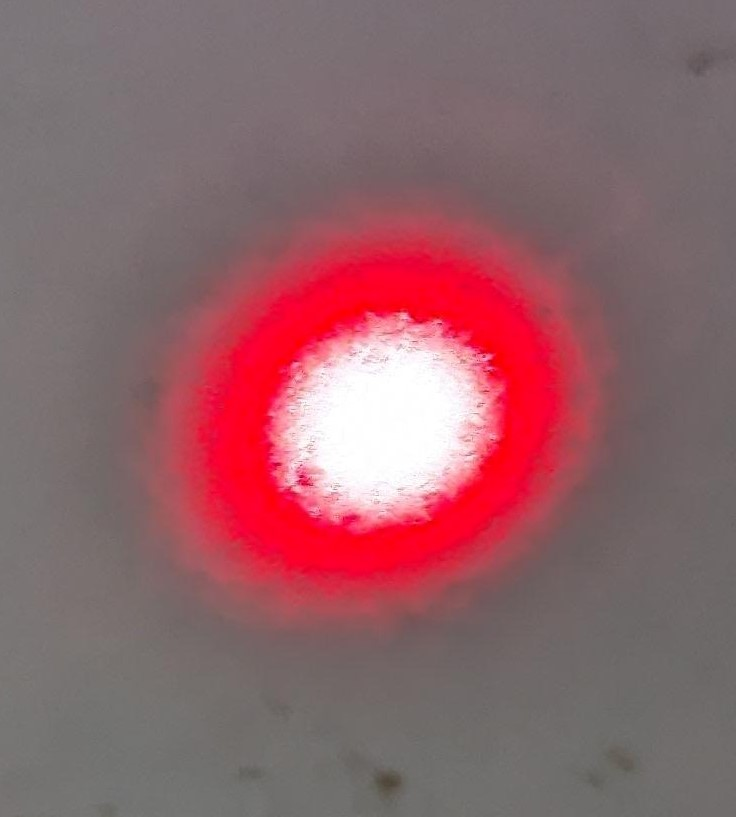
\includegraphics[width=0.28\textwidth]{Bilder/single_mode_fiber.jpg}
    }
  \subfloat[Multi-mode]{
        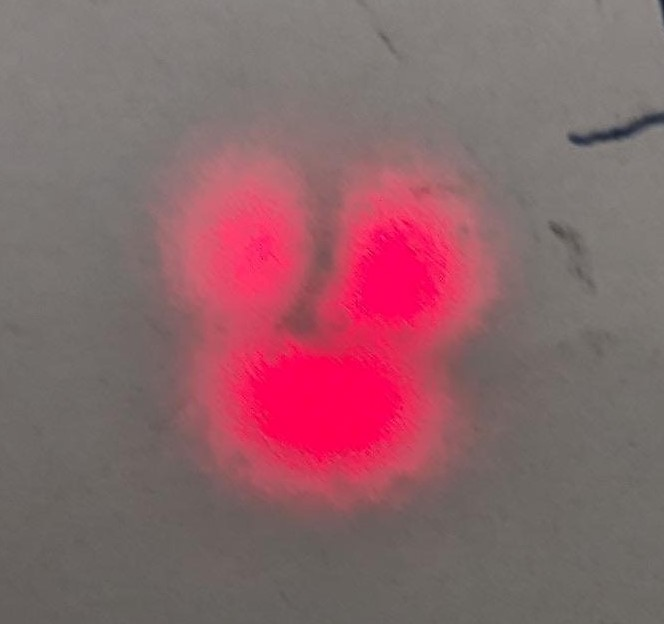
\includegraphics[width=0.28\textwidth]{Bilder/multi_mode_fiber.jpg}
    }\\
   \caption{Transmittierte Moden nach Glasfasern hinter $f=50\ \mathrm{mm}$ Linse}
    \label{FotostreckeGlasfasern}
\end{figure}
\subsection{Untersuchung eines Gaußschen Laserstrahls}

\subsubsection{Vermessung der Strahltaille}


%und daraus folgt
%\begin{equation}
%\frac{w_1^2}{w_2^2}=\frac{1+z_1^2/z_R^2}{1+z_2^2/z_R^2}\Rightarrow z_R=\sqrt{\frac{z_1^2-\frac{w_1^2}{w_2^2}z_2^2}{\frac{w_1^2}{w_2^2}-1}}.
%\end{equation}
%Mithilfe des so bestimmten Wertes kann $w_0$ bestimmt werden. 
%\begin{equation}
%w_0=\frac{w_i}{\sqrt{1+\frac{z_i^2}{z_R^2}}},\ i\in\{1,2 \}
%\end{equation}
\subsubsection{Vermessung des Strahlprofils hinter einer Konvexlinse}
Nun wurde eine Konvexlinse der Brennweite $f=100\ \mathrm{mm}$ in den Strahl gestellt. Diese führte zu einer deutlich schnelleren Aufweitung des Strahls im Vergleich zu dem Strahl, der den Faserkoppler verlässt. \\
Für verschiedene $z$ wurde der Strahldurchmesser $w(z)$ bestimmt. Das Vorgehen ist identisch zu dem beim Vermessen der Strahltaille. Mittels Gleichung \ref{w(z)} kann nun eine Anpassung an die gemessenen Werte vorgenommen werden. Die Regressionsfunktion lautet also:
\begin{equation}\label{w(z)}
w(z)=w_0\sqrt{1+\frac{(z-z_0)^2}{z_R(w_0)^2}},\ (z_0,w_0)\in \R\times\R^+
\end{equation}
\subsection{Optischer Resonator}

\subsubsection{Justieren und Bestimmen der Transmissionsfunktion}
\begin{figure}[H]

    \centering
    \subfloat[gestörte Transmissionsfunktion]{
        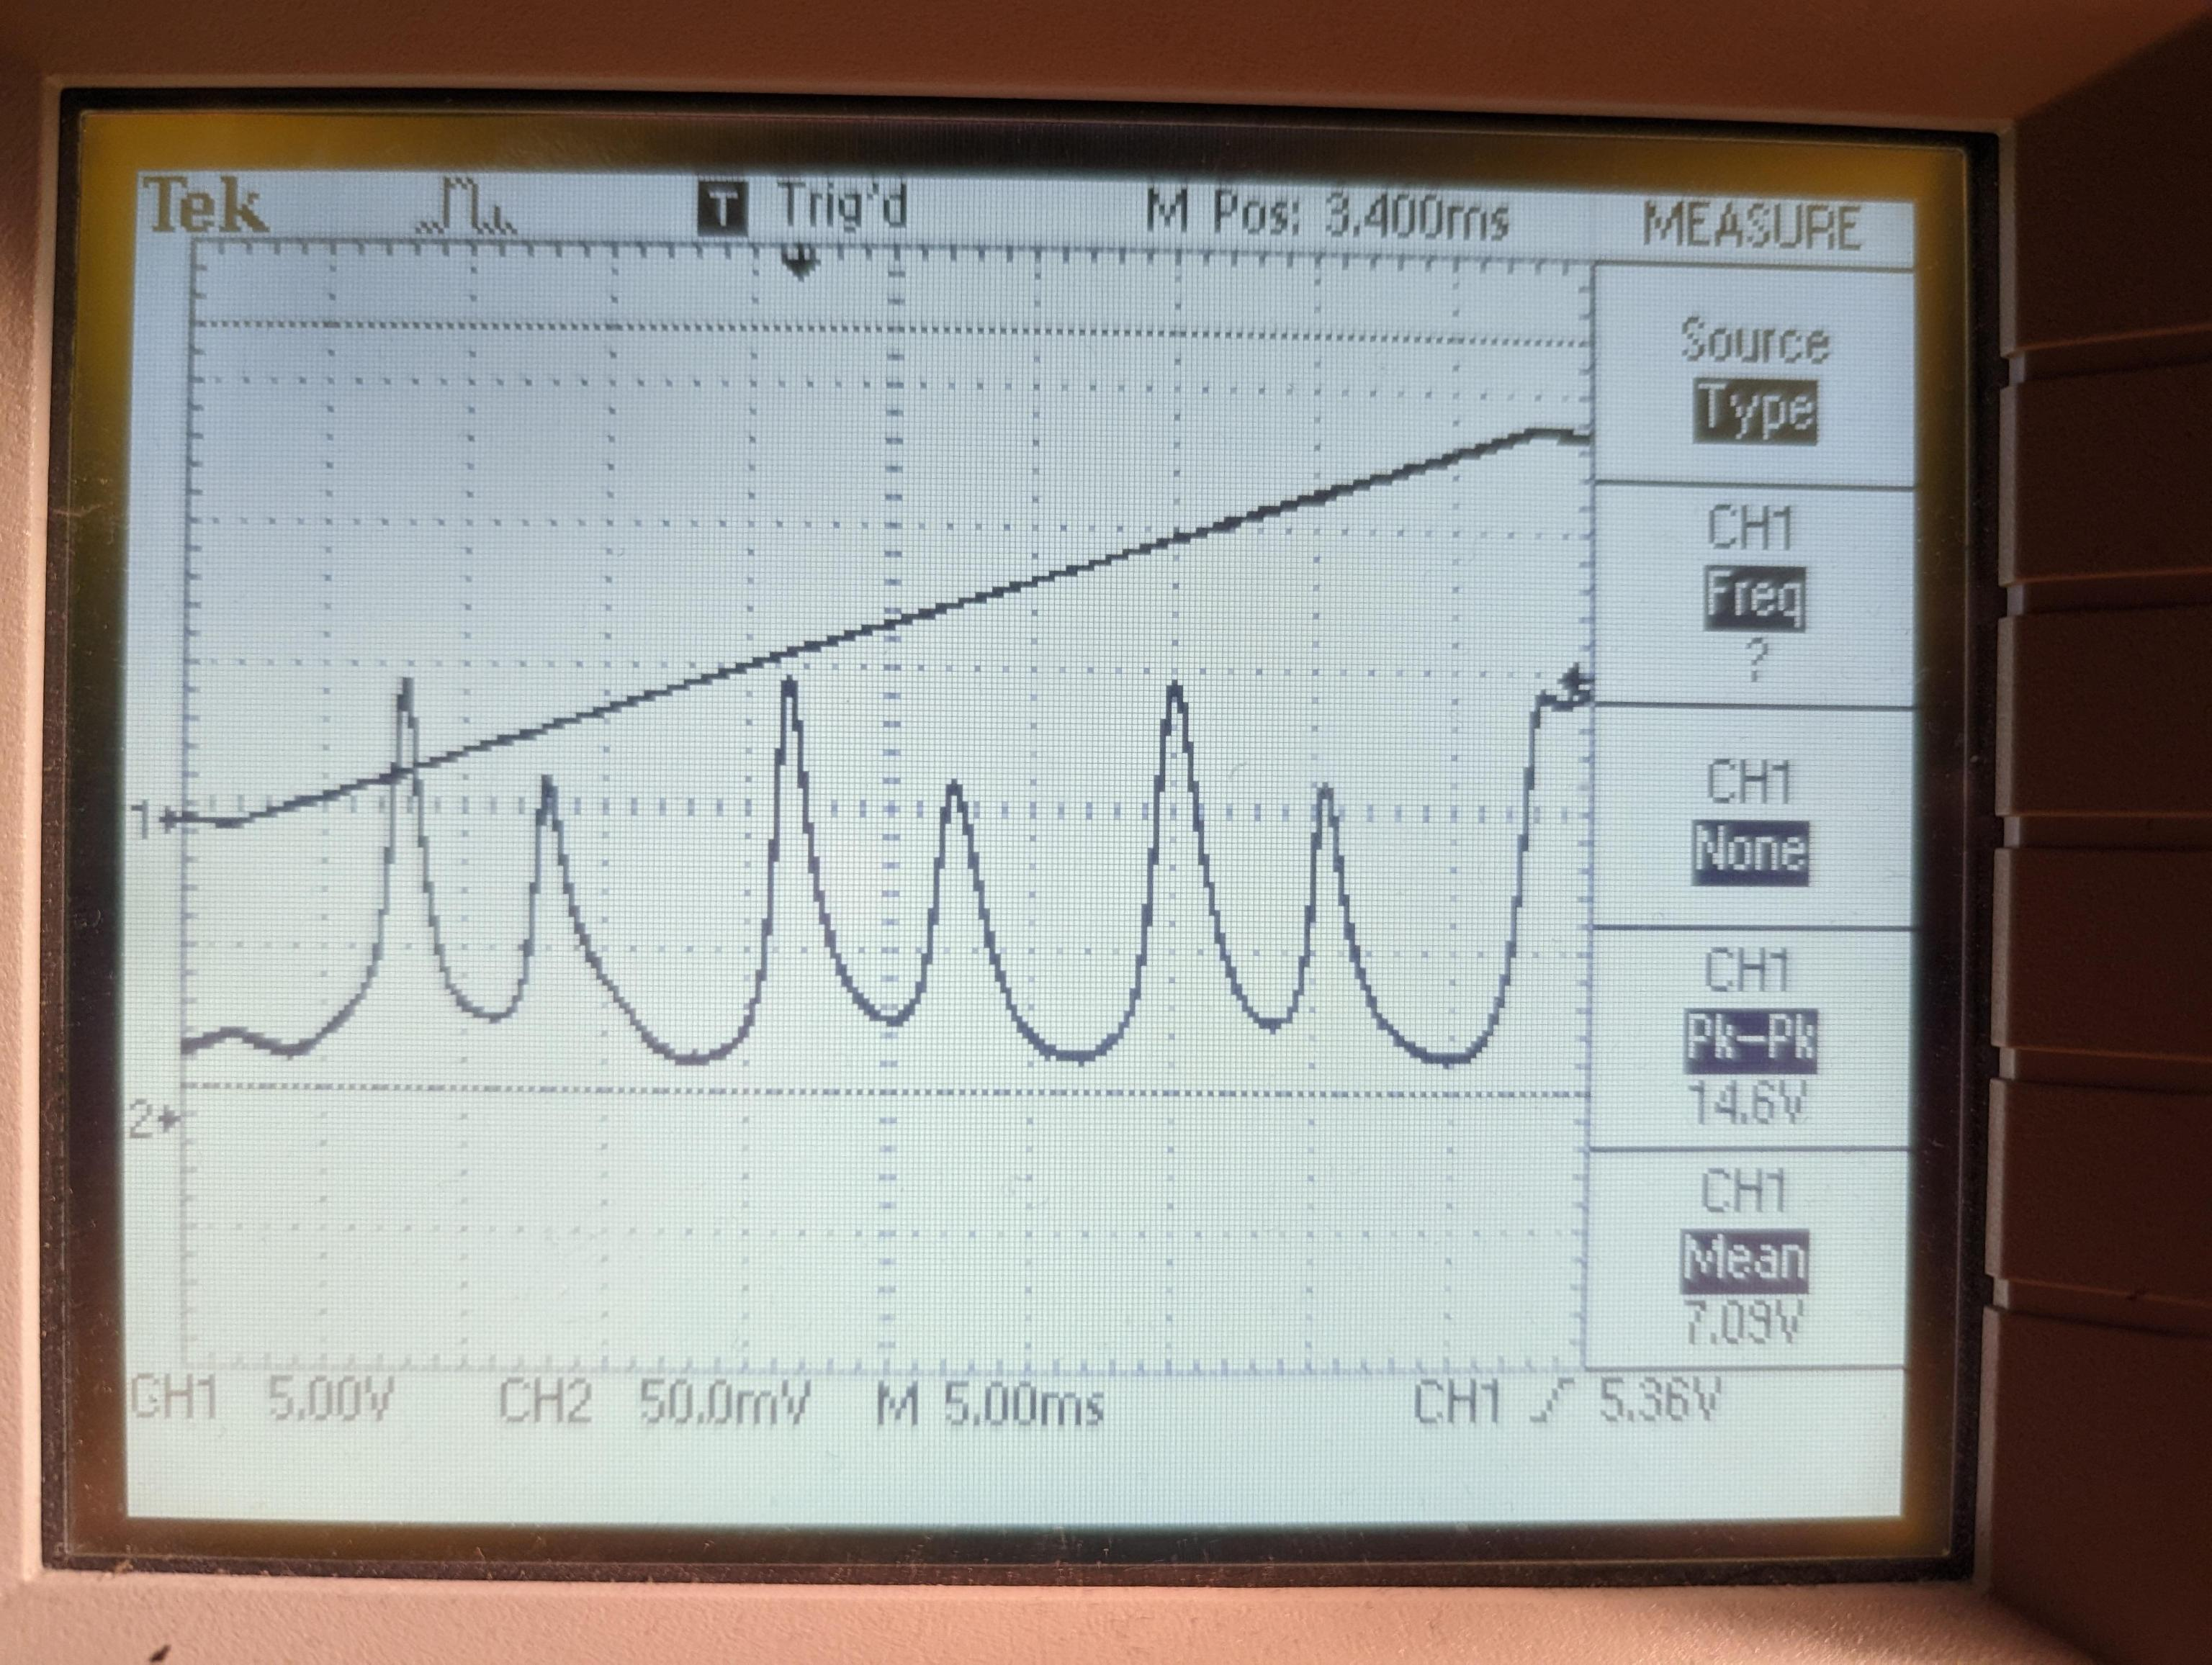
\includegraphics[width=0.4\textwidth]{Bilder/Osc_disturbed.jpg}
    }
  \subfloat[ungestörte Transmissionsfunktion]{
        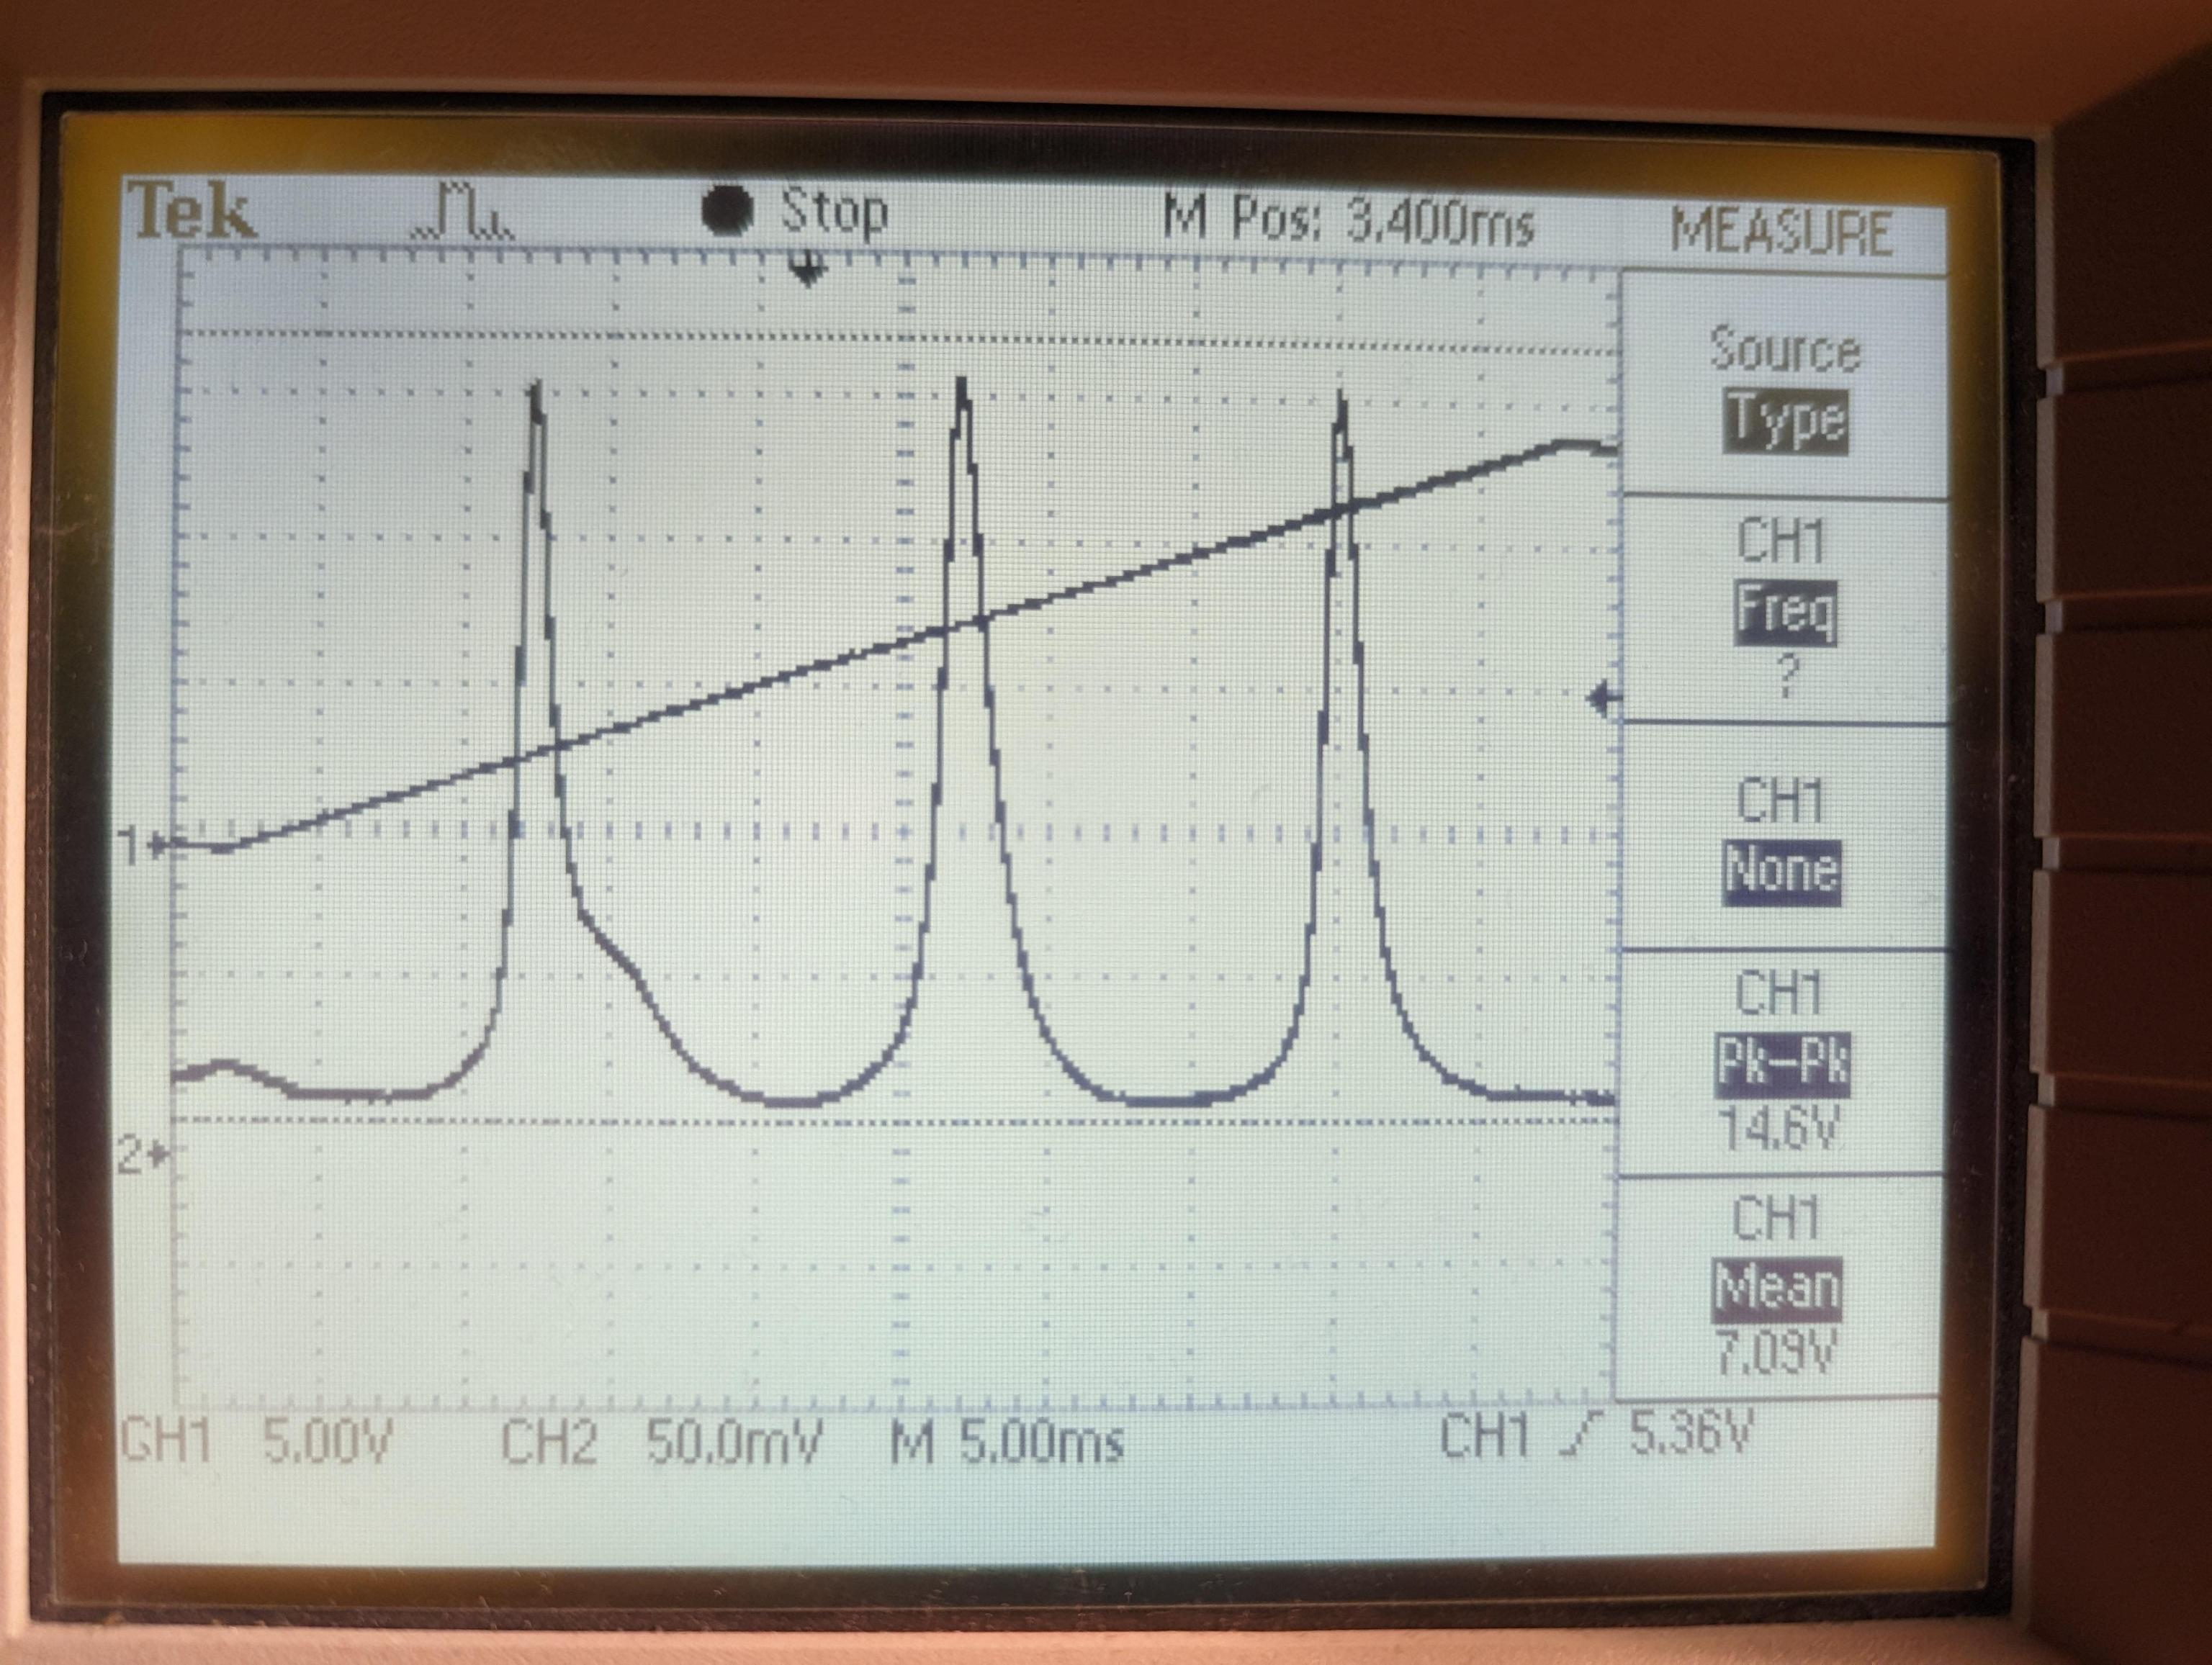
\includegraphics[width=0.4\textwidth]{Bilder/Osc_nice.jpg}
    }\\
   \caption{Transmissionsfunktion des konfokalen Resonators}
    \label{FotostreckeTransmissionsfunktion}
\end{figure}
%Berücksichtige nun die Linse zur Modenanpassung und deren Abstand $\mathfrak{d}$ zum Resonator.

\section{Ergebnisse und Diskussion}
\subsection{Bestimmung der Laserleistung und der Hintergrundhelligkeit}
Geht man bei der Photodiode von einem Quantenwirkungsgrad $\eta=75\%$ aus, so ergibt sich unter Ausnutzung der Propotionalität von Photostrom und einfallender Lichtleistung der folgende Zusammenhang zwischen der Laserleistung $P$ und der gemessenen Spannung:
\begin{equation}\label{P_diode}
P=\frac{hcU}{e\lambda\eta R}
\end{equation}
Dabei bezeichnet $h$ das Plancksche Wirkungsquantum, $e$ die Elementarladung, $c$ die Lichtgeschwindigkeit und $\lambda$ die mittlere Wellenlänge des einfallenden Lichtes. Beim Laser kann $\lambda_L=632.8\ \mathrm{nm}$ als fehlerfrei angenommen werden. Bei der Hintergrundhelligkeit wird $\lambda_R=(600\pm 100)\ \mathrm{nm}$ gesetzt.
Damit ergeben sich die folgenden Werte:\\
\begin{table}[H]
\centering
\begin{tabular}{@{}lllll@{}}
\toprule
                        & $\lambda$   & $P [\mathrm{mW}]$  & $\Delta P[\mathrm{mW}]$ &  \\ \midrule
$U_{L,\mathrm{hell}}$   & $\lambda_L$ & $0.2597$           & $0.0006$                &  \\
$U_{L,\mathrm{dunkel}}$ & $\lambda_L$ & $0.2599$           & $0.0006$                &  \\
$U_{R,\mathrm{hell}}$   & $\lambda_R$ & $1.4\cdot 10^{-3}$ & $0.3\cdot 10^{-3}$      &  \\
$U_{L,\mathrm{dunkel}}$ & $\lambda_R$ & $42\cdot 10^{-6}$  & $6\cdot10^{-6}$         &  \\ \bottomrule
\end{tabular}
\caption{Lichtleistungen im hellen/ dunklen Raum, mit/ ohne Laser}
\end{table}
Die Unsicherheiten wurden mit der MinMax-Methode abgeschätzt.\\
Insbesondere kann festgehalten werden, dass ein Vernachlässigen der Hintergrundstrahlung bei den anderen Teilversuchen gerechtfertigt ist, da während der Versuchsdurchführung im abgedunkelten Raum gearbeitet wurde. Die Werte für die Leistung des Lasers erscheint realistisch, da die Sollleistung des Lasers $1\ \mathrm{mW}$ beträgt und am Strahlteiler, an der Linse und am Spiegel Verluste durch Absorption oder Sekundärreflexionen auftreten.\\
Ferner kann die Intensität an der Tischoberfläche berechnet werden, indem die aktive Fläche der Photodiode auf $A=(3\pm1)^2\mathrm{mm}^2$ geschätzt wird. Folglich ergibt sich mit $I=\frac{P_{R,\mathrm{hell}}}{A}=(0.15\pm0.09)\frac{\mathrm{W}}{\mathrm m^2}$ ein ungenauer, aber realistisch erscheinender Wert. \\
Eine Verbesserung der Messgenauigkeit könnte durch Berücksichtigen der verschiedenenen des einfallenden Wellenlängenspektrums, das in guter Näherung dem der Sonne gleichen sollte, erzielt werden.
\subsection{Untersuchung eines Gaußschen Laserstrahls}
\subsubsection{Vermessung der Strahltaille}
Die gemessene Lichtleistung ist 
\begin{align}
P(x)&=\int_{-\infty}^\infty \mathrm dy^\prime \int_x^\infty \mathrm dx^\prime I_0\cdot\mathrm{exp}\left(-\frac{2(x^\prime-x_0)^2}{w^2}-\frac{2(y^\prime-y_0)^2}{w^2}\right) \\ \quad& = \sqrt{\frac{\pi}{2}}wI_0\int_x^\infty \mathrm dx^\prime \mathrm{exp}\left(-\frac{2(x^\prime-x_0)^2}{w^2}\right) \undereq{CAS}\hdots \\ \quad& =I_0\sqrt{\frac{\pi}{8}}w\cdot\left(\mathrm{erf}\left(\frac{\sqrt{2}}{w}(x_0-x)\right)+1\right)\\ \quad& \equiv \mathfrak{P}_0\cdot\left(\mathrm{erf}\left(\frac{\sqrt{2}}{w}(x_0-x)\right)+1\right)
\end{align}
Entsprechend können die Messdaten durch Anpassung der Parameter $(\mathfrak P_0,w,x_0)\in \R\setminus\{0\}\times\R^+\times\R$ gefittet werden.
Es ergibt sich \plotref{erf}
%\plot{erf}{Regression der gemessenen Strahltaille mit einer Fehlerfunktion}{1}{erf.pdf}
\subsubsection{Abschätzung der Parameter des kollimierten Laserstrahls}
Um einen groben Schätzwert für den Waistparameter $w_0$ zu erhalten, werden für vier verschiedene $z$ die Strahldurchmesser $w$ bestimmt. $z$ wird dabei ausgehend vom Faserende gemessen. \\
Es gilt dann allgemein
\begin{equation}\label{w(z)}
w(z)=w_0\sqrt{1+\frac{(z-z_0)^2}{z_R^2}}=\sqrt{w_0^2+\frac{(z-z_0)^2\lambda^2}{\pi^2n^2w_0^2}}
\end{equation}
gemäß den Gleichungen \ref{rayleigh} und \ref{transv_profil}. 
\subsubsection{Abschätzung der Parameter des kollimierten Laserstrahls}
\plot{coll_z}{transversales Strahlprofil des kollmierten Strahls}{1}{Messdaten Errorfunktion/w_z_data_coll.pdf}
\subsubsection{Vermessung des Strahlprofils hinter einer Konvexlinse}
\plot{div_z}{transversales Strahlprofil hinter $f=100\ \mathrm{mm}$ Linse}{1}{Messdaten Errorfunktion/w_z_data_div.pdf}
\subsection{Optischer Resonator}
\subsubsection{Bestimmung der Finesse}
Das Spektrum wurde in Form eines Fotos des Oszilloskopdisplays aufgenommen. Dieses Foto weist natürlich eine Parallaxe auf, d.h. das Display erscheint auf dem Foto verzerrt. Durch Anwenden einer linearen Transformation im Bildbearbeitungsprogramm GIMP kann das Bild entzerrt werden. Auf dem entzerrten Bild können pixelgenau die Abstände der Maxima und die FWHM-Breiten bestimmt werden. Da drei Maxima zu sehen sind, ergibt dies drei Werte für $\Delta\omega_{\mathrm{FWHM}}$ und zwei Werte für $\Delta\omega_{\mathrm{FSR}}$, aus denen je das arithmetische Mittel gebildet wird, dessen Unsicherheit über die empirische Standardabweichung abgeschätzt werden kann.\\
Man erhält auf diese Weise die Werte $\Delta\overline\omega_{\mathrm{FWHM}}=(101\pm13)\mathrm{px}$ und $\Delta\overline\omega_{\mathrm{FSR}}=(850\pm50)\mathrm{px}$. Dabei ist $1\mathrm{px}\propto 1\mathrm s$, da das untersuchte Bild entzerrt ist. \\
Es ergibt sich somit für die Finesse:
\begin{equation}
F_1\equiv \frac{\Delta\overline\omega_{\mathrm{FSR}}}{\Delta\overline\omega_{\mathrm{FWHM}}}=8.4\pm1.5
\end{equation}
Alternativ kann die Finesse unter Benutzung von Gleichung \ref{finesse_theor} und den gemessenen Transmissivitäten der beiden halbdurchlässigen Spiegel des Resonators berechnet werden. Dabei wird Absorption in den Spiegeln vernachlässigt, d.h. $R_i+T_i=1,\ i\in\{1,2\}$. Weiterhin ist $T_i=\frac{U_i}{U_{\mathrm{ohne}\ \mathrm{Spiegel}}}$. Dann folgt mittels Gaußscher Fehlerfortpflanzung \begin{equation}
\Delta F = \sqrt{\left(\frac{\partial F}{\partial U_1}\Delta U_1\right)^2+\left(\frac{\partial F}{\partial U_2}\Delta U_2\right)^2+\left(\frac{\partial F}{\partial U_{\mathrm{ohne}\ \mathrm{Spiegel}}}\Delta U_{\mathrm{ohne}\ \mathrm{Spiegel}}\right)^2}
\end{equation}
\section{Zusammenfassung}
\newpage

\bibliography{literatur} 
\bibliographystyle{ieeetr}
\appendix

\section{Python-Skripte zur Auswertung}
\subsection{Bestimmung des axialen Strahlprofils}
%\large\textbf{Code 1 zu Plot TV5:}
\lstinputlisting{Messdaten Errorfunktion/Erf_plot.py}
\subsection{Bestimmung des transversalen Strahlprofils ohne Linse}
\lstinputlisting{Messdaten Errorfunktion/w_z_plot_coll.py}
\subsection{Bestimmung des transversalen Strahlprofils mit Linse}
\lstinputlisting{Messdaten Errorfunktion/w_z_plot_div.py}
%\large\textbf{Code 2 zu Plot TV5:}
%\lstinputlisting{TV5_2.py}\newpage
\section{Plots zur Vermessung des Strahldurchmessers}
\subsection{Ohne Linse (kollimiert)}
\plot{coll_z_75}{axiales Strahlprofil bei $z=75\mathrm{mm}$}{.8}{Messdaten Errorfunktion/Collimated_z_75.pdf}
\plot{coll_z_150}{axiales Strahlprofil bei $z=150\mathrm{mm}$}{.8}{Messdaten Errorfunktion/Collimated_z_150.pdf}
\plot{coll_z_250}{axiales Strahlprofil bei $z=250\mathrm{mm}$}{.8}{Messdaten Errorfunktion/Collimated_z_250.pdf}
\plot{coll_z_350}{axiales Strahlprofil bei $z=350\mathrm{mm}$}{.8}{Messdaten Errorfunktion/Collimated_z_350.pdf}
\subsection{Mit Linse (fokussiert)}
\plot{div_z_75}{axiales Strahlprofil bei $z=75\mathrm{mm}$}{.8}{Messdaten Errorfunktion/Divergent_z_75.pdf}
\plot{div_z_50}{axiales Strahlprofil bei $z=50\mathrm{mm}$}{.8}{Messdaten Errorfunktion/Divergent_z_50.pdf}
\plot{div_z_175}{axiales Strahlprofil bei $z=175\mathrm{mm}$}{.8}{Messdaten Errorfunktion/Divergent_z_175.pdf}
\plot{div_z_250}{axiales Strahlprofil bei $z=250\mathrm{mm}$}{.8}{Messdaten Errorfunktion/Divergent_z_250.pdf}
\plot{div_z_100}{axiales Strahlprofil bei $z=100\mathrm{mm}$}{.8}{Messdaten Errorfunktion/Divergent_z_100.pdf}
\plot{div_z_125}{axiales Strahlprofil bei $z=125\mathrm{mm}$}{.8}{Messdaten Errorfunktion/Divergent_z_125.pdf}


\end{document}